\documentclass[11pt]{article}
\usepackage[top=1in, bottom=0.5in, left=1in, right=1in]{geometry}
\usepackage[T1]{fontenc}
\usepackage[polish]{babel}
\usepackage[utf8]{inputenc}
\usepackage{lmodern}
\selectlanguage{polish}
\usepackage{graphicx}
\begin{document}
\title{Laboratorium 4}
\author{Jan Seredyński}
\date{\today}
\maketitle

\section{Wstęp}
Zadaniem laboratorium jest pomiar czasu wykonania operacji wypelnienia tablicy asocjacyjnej (słownika). Do wykonania analizy zstosowałem wcześniej przygotowaną listę dwukierunkową(nie opartą na tablicy).


\section{Moja implementacja słownika}
Przy utworzenia klasy słownik uznałem, że najważniejszą metodą którą się używa jest operator[], więc pełni on główną rolę w moim kodzie. Dzięki niemu możemy zapisywać oraz odczytywać elementy z tablicy dzięki zastosowaniu referencji.

\section{Wydajność słownika}
Wykorzystałem metode łańcuchową transformacji kluczowej, której idee pokazuje obraz poniżej.
\par\vspace{\baselineskip}
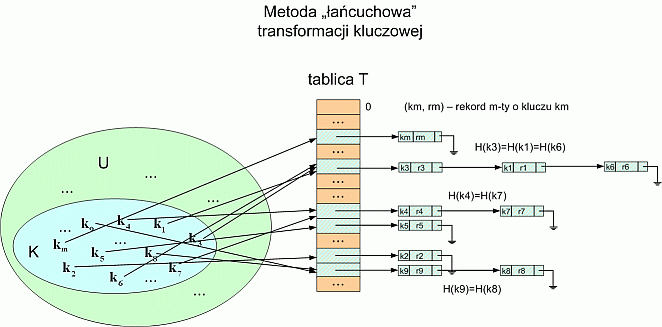
\includegraphics[width=5in]{lancuchowa.png}\\\
W mojej implementacji złożoność obliczeniowa słownika wynosi $O(n*log^n)$),co można zaobserwować na wykresie poniżej.\\\
Do testów napisałem oddzielny modul generujący losowe wyrazy i liczby, które nastepnie zapisuje do słownika.
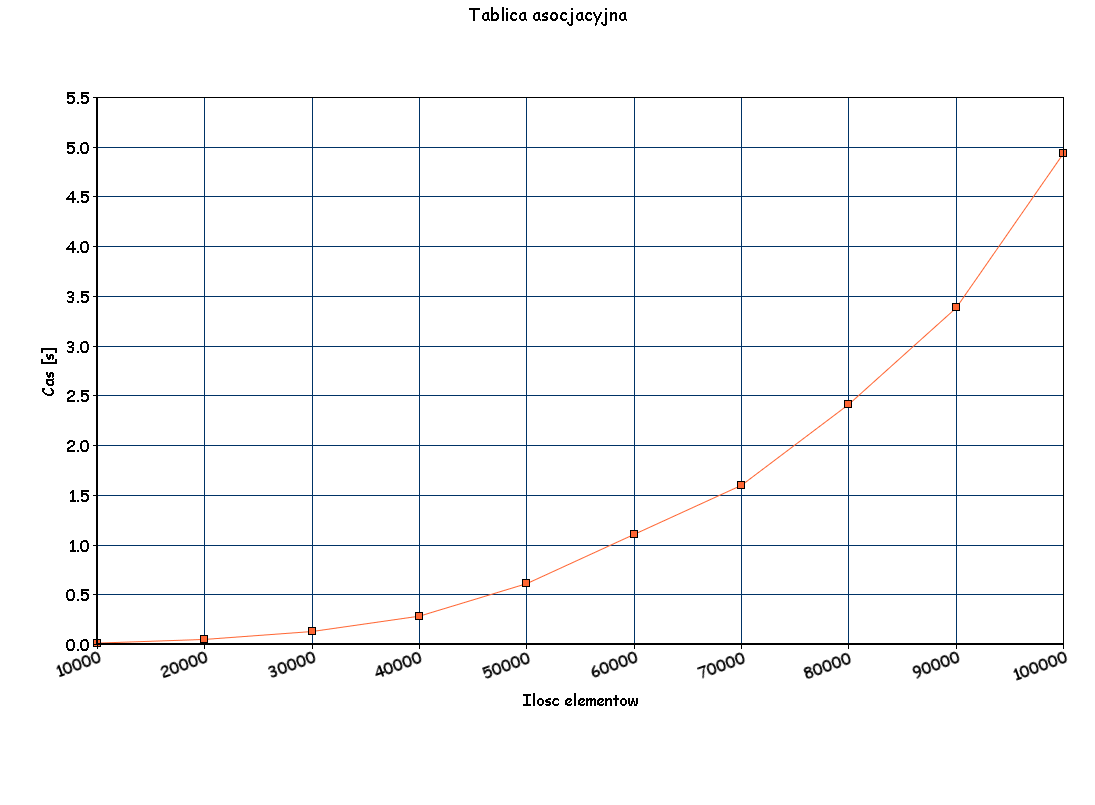
\includegraphics[width=6in]{slownik.png}


\section{Podsumowanie}
Mógłbym ulepszyć moją tablice asocjacyjną poprzez zrobienie jej na liscie opartej na tablicy i zastosowainu sortowania binarnego.
Kolejnym ulepszeniem byłoby ulepszenie mojej implementacji listy, tak aby mogła wyszukiwać elementy w liscie bez potrzeby popowania wczesniejszych elementów.
\end{document}